% Note to reader: lines beginning with the '%' character are
% 'comments' to you, the human reader of this code, and are 
% ignored by the LaTeX compiler.

%%%%%%%%%%%%%%%%%%%%%%%%%%%%%%%%%%%%%%%%%%%%%%%%%%%%%%%%%%%%%%%%%%
% = Sample template for MIT Junior Lab Student Written Summaries =
% Available from 
%    http://web.mit.edu/8.13/www/Samplepaper/sample-paper.tex
%
% Last Updated July 23, 2014
%
% Adapted from the American Physical Societies REVTeK-4.1 Pages
%    at http://publish.aps.org
%
% ADVICE TO STUDENTS: Each time you write a paper, start with this
%    template and save under a new filename.  If convenient, don't
%    erase unneeded lines, just comment them out using the 
%    '%' character at the start of the line.  Often, they
%    will be useful containers for information.
%
% Using pdflatex, images must be either PNG, GIF, JPEG or PDF.
%    Turn EPS (encapsulated postscript) images to PDF using the
%    epstopdf utility on UNIX systems.
%%%%%%%%%%%%%%%%%%%%%%%%%%%%%%%%%%%%%%%%%%%%%%%%%%%%%%%%%%%%%%%%%%

%%%%%%%%%%%%%%%%%%%%%%%%%%%%%%%%%%%%%%%%%%%%%%%%%%%%%%%%%%%%%%%%%%
% = TO COMPILE THIS DOCUMENT =
%
% From the command line, it would go like this --- assuming you are
%    in the directory where the filename.tex source file and the 
%    filename.bib bibliography file are located, and that you have 
%    permission to create and write files in that directory:
%      > pdflatex filename
%      > bibtex filename
%      > pdflatex filname
%      > pdflatex filename
%    Yes, you run the command several times. The earlier runs 
%    create auxilliary files which keep track of references,
%    citations, equation and section numberring, etc. The later
%    runs combine the information in these auxilliary files with
%    your source document to create the finished product.
%
% If you are using a GUI LaTeX editor like TeXWorks, then there
%    is probably a menu bar button for pdfLaTeX and another for
%    BibTeX. Hit them in the order indicated above. There is 
%    probably also a 'TeXify' button, or something similarly named,
%    which runs all the above commands in one shot.     
%%%%%%%%%%%%%%%%%%%%%%%%%%%%%%%%%%%%%%%%%%%%%%%%%%%%%%%%%%%%%%%%%%


%%%%%%%%%%%%%%%%%%%%%%%%%%%%%%%%%%%%%%%%%%%%%%%%%%%%%%%%%%%%%%%%%%
%  = PREAMBLE =
% The preamble of a LaTeX document is the set of commands that precede
% the \begin{document} line.  It contains a \documentclass line
% to load the REVTeK-4.1 macro definitions and various \usepackage
% lines to load other macro packages.
%
% ADVICE TO STUDENTS: This preamble contains a suggested set of
%     class options to generate a ``Junior Lab'' look and feel that
%     facilitate quick review and feedback from one's peers, TAs,
%     and section instructors.  Don't make substantial changes 
%     to the style without first consulting your section 
%     instructor.
%%%%%%%%%%%%%%%%%%%%%%%%%%%%%%%%%%%%%%%%%%%%%%%%%%%%%%%%%%%%%%%%%%

%\documentclass[aps,twocolumn,secnumarabic,balancelastpage,amsmath,amssymb,nofootinbib, floatfix]{revtex4}
\documentclass[aps,twocolumn,nobalancelastpage,secnumarabic,amsmath,amssymb,nofootinbib,floatfix]{revtex4-1}

%%%%%%%%%%%%%%%%%%%%%%%%%%%%%%%%%%%%%%%%%%%%%%%%%%%%%%%%%%%%%%%%%%%
% N.B.:  Different computers have different packages installed.  
%        To compile this template in the current Athena 
%        environment, REVTeX 4.1 must be used.  To use the older
%        REVTeX 4, switch which documentclass line above is 
%        commented out above. There are ``bad'' distributions of
%        LaTeX for Windows available on the internet which may 
%        cause users to struggle unjustifiably with REVTeX 4.1.
%
%        If you are unable to compile the template at all, you
%        may need to update your LaTeX packages. (Alternatively, if 
%        your LaTeX distribution includes only the older RevTEX 4,
%        then try changing the documentclass line above. In particular,
%        this approach solves a common compilation problem for users of
%        the TeXWorks editor on Windows, which presents erroneously as a
%        error in the bibliography file.) Don't hesitate to speak 
%        with your section instructor or a TA if you're having 
%        issues getting this template to compile.
%%%%%%%%%%%%%%%%%%%%%%%%%%%%%%%%%%%%%%%%%%%%%%%%%%%%%%%%%%%%%%%%%%%

%%%%%%%%%%%%%%%%%%%%%%%%%%%%%%%%%%%%%%%%%%%%%%%%%%%%%%%%%%%%%%%%%%%
% = Explanation of documentclass options =
%
% aps, prl stand for American Physical Society and Physical 
%     Review Letters respectively.
% twocolumn permits two columns, of course.
% nobalancelastpage doesn't attempt to equalize the lengths of 
%     the two columns on the last page  as might be desired in a 
%     journal where articles follow one another closely.
% amsmath and amssymb are necessary for the subequations 
%     environment among others. These functionalities can
%     also be added use the usepackage function described below,
%     but REVTeX conveniently includes them as documentclass
%     options.
% secnumarabic identifies sections by number to aid electronic 
%     review and commentary.
% nofootinbib forces footnotes to occur on the page where they are
%      first referenced and not in the bibliography.
% floatfix attempts to help LaTeX decide where to place ``floats'',
%      like figures and plots, when it gets stuck and can't decide
%      by it's normal algorithm.
% REVTeX 4.1 is a set of macro packages designed to be used with 
%      LaTeX 2e. REVTeX is well-suited for preparing manuscripts 
%      for submission to APS journals.
%
% = Other documentclasses =
%
% The 'revtex4' and 'revtex4-1' documentclasses are somewhat 
%    specialized for making documents in the style of the APS
%    journals. For a more standard or generic looking LaTeX paper,
%    you could try any of the built-in documentclasses, in 
%    particular 'article' or 'report'. Someday, you may try to use 
%    the 'mitthesis'  documentclass available for download from the 
%    MIT Libraries. The vast majority of source code written for 
%    one documentclass should work just fine in any other, but 
%    occasional quirks arise. For example, some documentclasses 
%    disagree on whether the abstract declaration should come 
%    before or after the \begin{document} declaration.
% 
%%%%%%%%%%%%%%%%%%%%%%%%%%%%%%%%%%%%%%%%%%%%%%%%%%%%%%%%%%%%%%%%%%%

%% Now, include some packages which provide new commands that 
%% extend LaTeX's capabilities. Note that the nearly-essential
%% AMS math packages were added already as documentclass options
%% for REVTeX, but could have been added here using 
%% \usepackage{amsmath}, etc. The pacakges below are commonly 
%% useful, but there are many, many more available to solve a 
%% multitude of typesetting quandries (google your problem), 
%% and you  probably have the necesary packages installed on your
%% system already. Among the examples listed below, this sample
%% document only actually makes use of the 'graphicx', 'bm', 
%% and 'hyperref' pacakges, so the others are commented out for
%% tidyness.


\usepackage{graphicx}      % tools for importing graphics
\usepackage{lipsum}
\usepackage{float}
%\usepackage{lgrind}        % convert program code listings to a form 
                            % includable in a LaTeX document
%\usepackage{xcolor}        % produces boxes or entire pages with 
                            % colored backgrounds
%\usepackage{longtable}     % helps with long table options
%\usepackage{epsf}          % old package handles encapsulated postscript issues
\usepackage{bm}            % special bold-math package. usge: \bm{mathsymbol}
\usepackage{physics}
\usepackage{tensor}
%\usepackage{asymptote}     % For typesetting of mathematical illustrations
%\usepackage{thumbpdf}
\usepackage[colorlinks=true]{hyperref}  % this package should be added after 
                                        % all others.
                                        % usage: \url{http://web.mit.edu/8.13}


%%%%%%%%%%%%%%%%%%%%%%%%%%%%%%%%%%%%%%%%%%%%%%%%%%%%%%%%%%%%%%%%%%%
% And now, begin the document...
%%%%%%%%%%%%%%%%%%%%%%%%%%%%%%%%%%%%%%%%%%%%%%%%%%%%%%%%%%%%%%%%%%%

\begin{document}
\title{Relativistic Behavior Detection through Electron Acceleration}
\author{Henry Shackleton}
\email{hshackle@mit.edu}
\date{\today}
\affiliation{MIT Department of Physics}


\begin{abstract}
  Classical and relativistic mechanics differ in their predictions of how the momentum of particles depend on their energy and velocity. By accelerating electrons emitted from a $\tensor*[^{90}]{\text{Sr}}{}$ source through a magnetic field, we are able to accurately measure these relations for the electrons. Using this, we are able to conclude that the relativistic theory better predicts the trends measured. Additionally, fitting these relations allows us to determine the electron charge as $(5.0 \pm 0.3) \times 10^{-10}$ esu, the electron rest energy as $(5.05 \pm 0.76) \times 10^{2}$ kEv, and the electron mass as $(1.07 \pm 0.23) \times 10^{-27}$ g.
\end{abstract}

\maketitle
\section{Introduction and Theory}
Albert Einstein's 1905 paper, ``On the Electrodynamics of Moving Bodies," was one of the foundational papers to developing the theory of special relativity. This theory was intended to reconcile inconsistencies with classical mechanics, electrodynamics, and observed phenomena. In his paper, Einstein postulated that the speed of light is a constant value in all reference frames, contradicting the classical prediction that light appears to travel faster or slower depending on one's speed relative to the light \cite{einstein}. This postulate leads to a new theory of dynamics, with different predictions than classical mechanics. We determine which theory gives more accurate predictions by examining electrons at speeds close to the speed of light - the regime where classical and relativistic theories differ the most.

In classical mechanics, the kinetic energy $K$ of a particle as a function of momentum $p$ is given by
\begin{equation}
  K = \frac{p^2}{2m}
\end{equation}
where $m$ is the mass of the particle. Most notably, the kinetic energy as a function of momentum is quadratic.
In special relativity, the kinetic energy of a particle as a function of momentum is instead given by
\begin{equation}
  K = \sqrt{p^2 c^2 + m^2c^4} - mc^2
\end{equation}
where $c$ is the speed of light - approximately $3.0 \times 10^{8}$ km/s. The value $mc^2$ is known as the \textit{rest energy} of a particle. When this rest energy is much larger than $pc$, this equation reduces to Equation $1$, as shown rigorously in Appendix A. For particles where the rest energy is small relative to $pc$, the first term in Equation $(2)$ dominates and $K$ becomes approximately a linear function of $p$. 

These predictions from classical mechanics and special relativity gives us two different relations, from which we can compare against our experimental data. The remainder of our analysis of the physical theory will be used to determine how the kinetic energy and momentum of a particle relate to our setup.

In our experiment, we will use a magnetic field to affect the trajectory of electrons - the particles whose relativistic effects we wish to detect. The Lorentz law is an equation that holds in both classical mechanics and special relativity, and determines how electric and magnetic fields affect the motion of a charged particle. In the presence of an electric field $\vb{E}$ and a magnetic field $\vb{B}$, the change in momentum is related to the two fields, the charge of the particle $e$, the velocity of the particle $\vb{v}$, and the speed of light $c$ by
\begin{equation}
    \dv{\vb{p}}{t} = e\left(\vb{E} + \frac{\vb{v}}{c} \times \vb{B} \right)
  \end{equation}
  Equation $(3)$ implies that charged particles subject to a constant magnetic field $B$ will move in orbits in the plane perpendicular to the magnetic field, with a radius of rotation $\rho$ proportional to the momentum of the particle.
  \begin{equation}
    p = \left(\frac{e\rho}{c}\right) B
  \end{equation}
Substituting this into our equations of kinetic energy, we see that the kinetic energy of a particle with charge $e$ and mass $m$ accelerated by a magnetic field $B$ around a radius $\rho$ is given by
\begin{equation}
  K = \frac{e^2 \rho^2}{2mc^2} B
\end{equation}
for classical mechanics, and
\begin{equation}
  K = \sqrt{e^2 \rho^2 B^2 + m^2 c^4} - mc^2
\end{equation}
for special relativity. The qualitative behavior of these equations are the same as Equations $1$ and $2$, but with different constants. By accelerating particles with a magnetic field at a fixed radius and measuring the kinetic energy of the particles, we can obtain an experimental graph of $K(B)$ which will allow us to compare our relativistic and non-relativistic models.
\section{Experimental Setup}
Our experimental setup consists of a large, spherical shell with coils wrapped around it. When these coils are fed a current, it generates an approximately uniform magnetic field across the inside of the shell, oriented vertically. By varying the current supplied to the coils, we can control the magnetic field inside the shell. The top and bottom hemispheres of the shell are disconnected, to allow for inspection of the internal components of the shell.

In the bottom hemisphere of the shell, a vacuum chamber is maintained through a mechanical pump and monitored by a pressure gauge. On one side of the chamber, a $\tensor*[^{90}]{\text{Sr}}{}$/$\tensor*[^{90}]{\text{Y}}{}$ beta source is placed. This beta source emits electrons with energies up to $2.28$ MeV. When electrons are emitted in the presence of the magnetic field, their trajectories are curved into orbits relative to their momentum, as predicted by Equation 4 and shown visually in Figure \ref{diagram}.

On the other side of the chamber, placed at a distance of $40.6 \pm 0.4$ cm away from the source, is a parallel-plate velocity selector and a PIN diode detector. When the electrons are accelerated in a helical orbit, only electrons of a certain momentum will pass between the two plates. If these electrons continue on their helical orbit, they will hit the side of the plates and not be detected by the PIN diode. By supplying a constant electric field $E$ between the two plates, the trajectory of the electrons can be straightened out and detected by the PIN diode by some $E$ proportional to the velocity of the electrons. This follows directly from the Lorentz law. When the electrons come in contact with the PIN diode, the kinetic energy is converted into an electric signal, which is fed through an amplifier and read by a multi-channel analyzer (MCA). This configuration allows us to detect the velocity, momentum, and kinetic energy of incoming electrons by looking at the supplied electric field, magnetic field, and MCA readout respectively.

Located halfway between the helical trajectory between the beta source and the detector is a metal divider with a small slit in it. In the absence of a perfect vacuum, our vacuum chamber will be filled with other particles, which the electrons from our beta source can scatter off of. To minimize the effects of this, we place a slit to attempt to screen our particles and only allow particles to pass through the slit whose trajectories have not been altered by scattering.

\begin{figure}[h]
  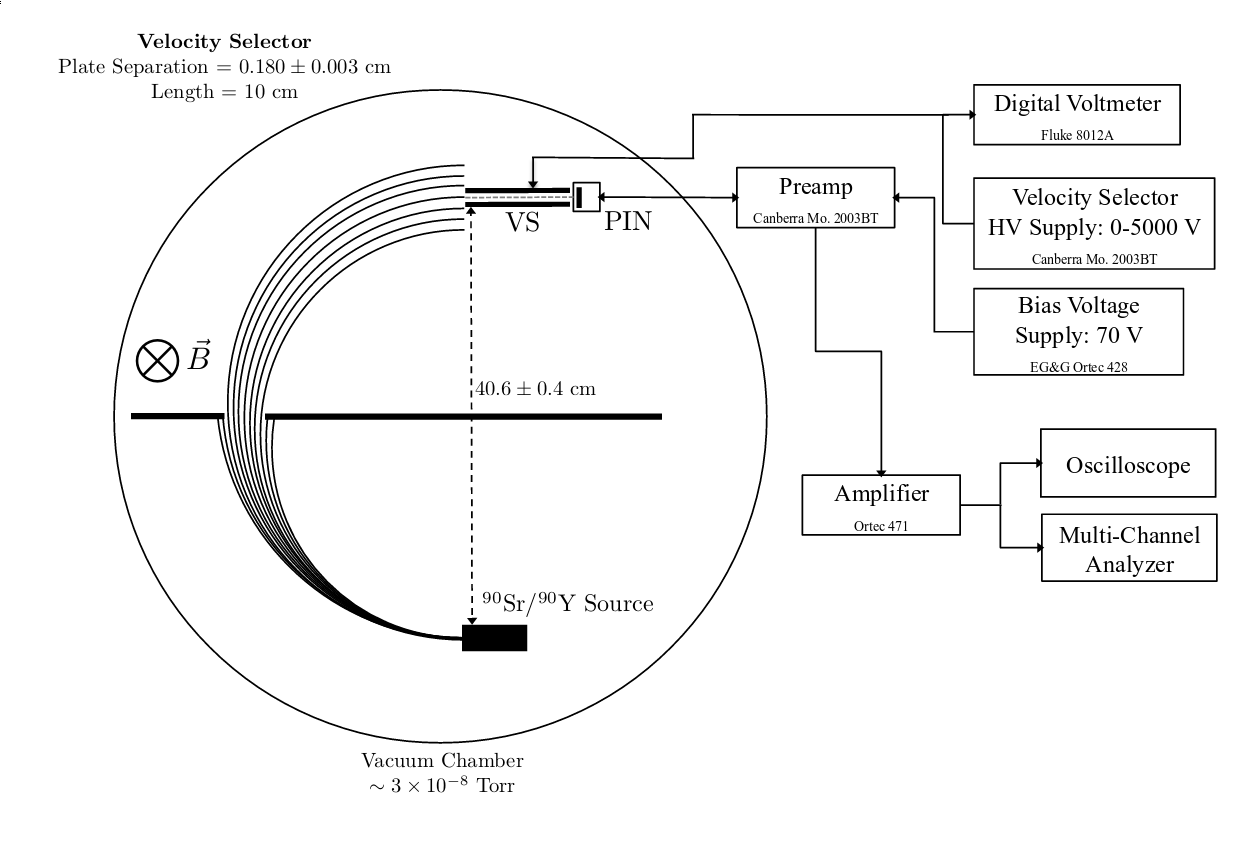
\includegraphics[width=.5\textwidth]{setup.png}
  \caption{A block diagram of our experimental setup. The circular lines drawn depict the expected trajectories from the beta source to the PIN diode detector. Signals from the PIN diode are amplified and sent to a Multi-Channel Analyzer, as well as an oscilloscope for troubleshooting. Our velocity selector is connected to a voltage supply, as well as a voltometer to measure the voltage supplied.
\cite{emanual}}
  \label{diagram}
\end{figure}

\section{Experimental Calibration}
Prior to our experiment, we carry out three calibration procedures - the MCA calibration, the magnetometer calibration, and inhomogeneity measurements of our magnetic field. The MCA calibration is necessary for our experiment, while the latter two calibrations are used to correct for systematic errors and obtain more accurate measurements.

The MCA detects the strength of incoming electric signals and bins them by their amplitude. This amplitude corresponds to the kinetic energy of the particles hitting the PIN diode, but the correspondence between the kinetic energy and the measured amplitude is initially unknown. To determine this relation, we place a $\tensor*[^{133}]{\text{Ba}}{}$ source next to the PIN diode. The spectrum of $\tensor*[^{133}]{\text{Ba}}{}$ is well known and can be used to calibrate our MCA. %Displayed in Figure $2$ is an example of an MCA readout of a $\tensor*[^{133}]{\text{Ba}}{}$ source, with various peaks labeled. In Table $1$, the energy known to correspond to these peaks is listed.
Using this data, we can calibrate our MCA to measure the kinetic energy of incoming electrons. This calibration comes with some uncertainty, but in our experiment, we determined this uncertainty to be negligible. 

To measure the magnetic field supplied to our electrons, we use a Hall effect magnetometer. To calibrate this magnetometer, we measure several sources with known magnetic fields. By comparing this data to the magnetic field displayed by the magnetometer, shown in Table \ref{magnetometer}, we are able to fit this relation to a linear equation $\text{B}_{actual} = (0.94 \pm 0.01)\text{B}_{measured} + (-0.02 \pm 0.09)$ that can be used to correct for systematic uncertainties in magnetic field measurement. 
\begin{table}[h]
\begin{tabular}{||c c||}
  \hline
      B$_{expected}$ (G)&B$_{measured}$ (G)\\
      \hline
      \hline
      $0.0$ & $0.0 \pm 0.1$ \\
      \hline
      $99.69 \pm 1.0$ & $111.3 \pm 0.2$ \\
      \hline
      $202.5 \pm 2.0$ & $201.5 \pm 0.2$ \\
      \hline
    \end{tabular}
  \caption{A comparison of expected magnetic field values from various sources and the measured values. As the measured value varied depending on the location, we set the magnetometer to ``peak hold," which displays only the largest value measured. We expect the location of the largest magnetic field to correspond to the location where the magnetic field is at the expected value.}
  \label{magnetometer}
\end{table}

The magnetic field generated by our device is assumed in our calculations to be homogeneous. However, this is not practically the case. To account for this, we measure the magnetic field at three different points along the trajectory. One of these points will be the location that we measure during our experimental runs. By averaging over these values, and repeating this measurement for various magnetic fields, we are able to obtain another linear relation which relates the magnetic field that we measure during our run to the average magnetic field across the trajectory of our electrons. This relation is given by a fit of $\text{B}_{average} = (0.99 \pm 0.01) \text{B}_{measured} + (0.81 \pm 0.99)$. These two relations - the inhomogeneity fit and the magnetometer fit - will be applied to our reported magnetic fields to acquire more accurate measurements, at the cost of some systematic uncertainty.
%\begin{figure}[h]
%  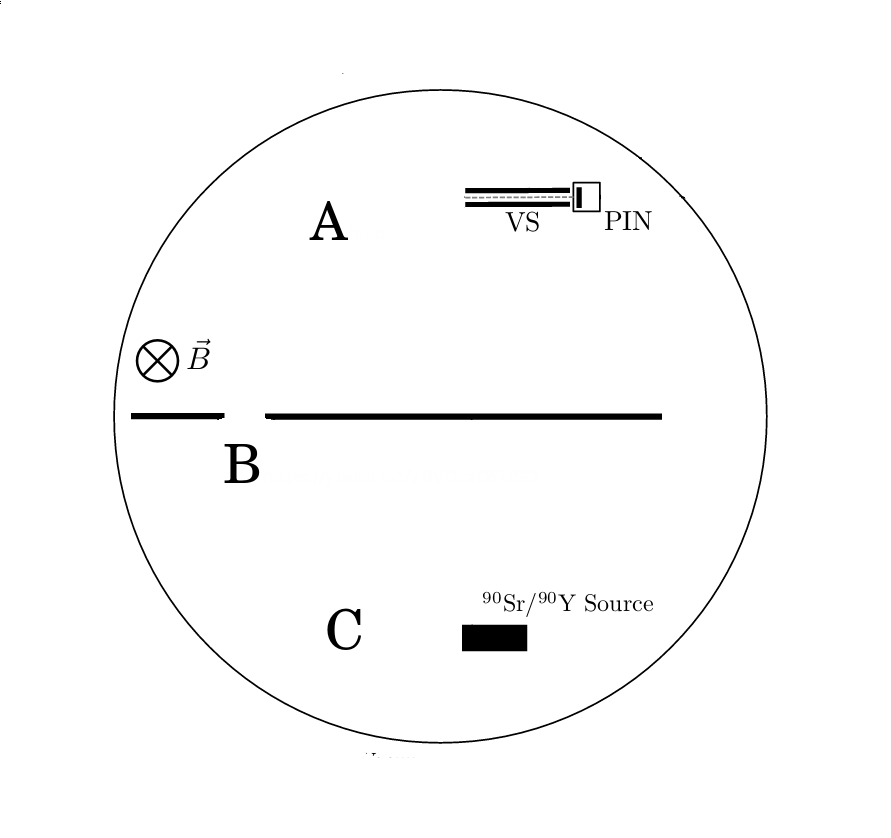
\includegraphics[width=.5\textwidth]{inhomo.png}
%  \caption{The three locations, labeled A, B, and C, where we measured the magnetic field inside our apparatus in order to determine the correspondence between the magnetic field at "C" - the location at which we will measure the magnetic field during our experimental run - and the average magnetic field across the electron trajectory}
%  \label{inhomo}
%\end{figure}
\section{Data Analysis}
In the course of our experiment, we collect data at four different values of the measured magnetic field, ranging from 90G to 120G in 10G increments. Note that this range only corresponds to the range of the magnetic fields displayed on the magnetometer - after correcting for the systematic uncertainties in the magnetometer and inhomogeneities in the magnetic field, the actual range of magnetic fields measured fall between 84G and 112G.

In each of the different values of the magnetic field, we conduct a sweep of voltages supplied to our parallel-plate velocity selector, which corresponds to a sweep of the electric field between the two plates. As previously detailed, we expect some value of the electric field, E$^*$,  to straighten out the trajectory of the electrons and result in peak detection. By sweeping through values of the electric field and measuring the number of counts received by the MCA, we are able to obtain an approximate value for E$^*$. This will allow us to calculate the velocity of our electrons at a given momenta, as well as the kinetic energy.

For each run of a specific magnetic and electric field, we allow the MCA to collect data for 315 seconds in real time. We obtain for each run a set of data, an example of which is shown in Figure \ref{mca}.

\begin{figure}[h]
  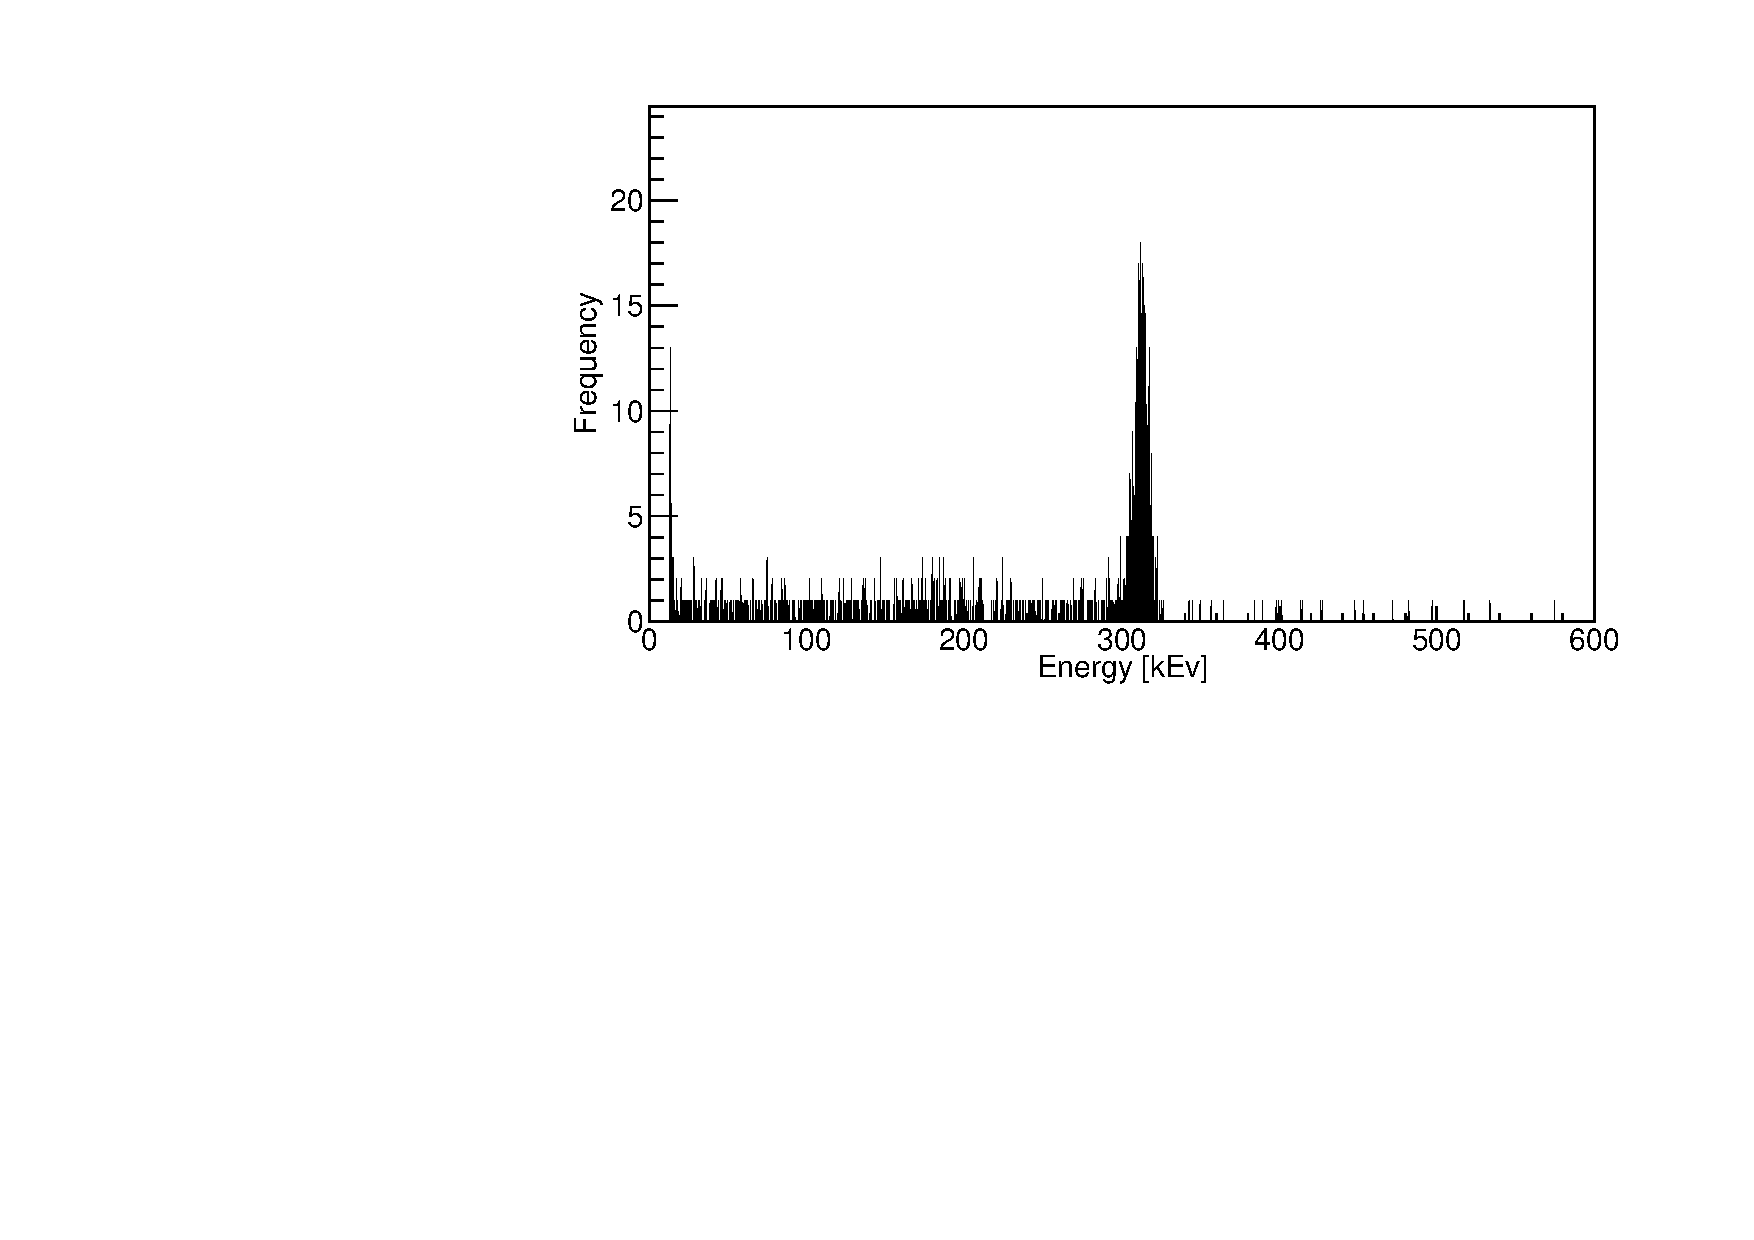
\includegraphics[width=.5\textwidth]{mca-readout-clean.pdf}
  \caption{Measured MCA detections for a single run, with $\text{B}_{measured} = 110$G and E $ = 4.4$kV. The MCA bins have been converted via the MCA calibration to their corresponding energies. The frequency of counts is sharply peaked around a small range of energies. We expect counts that fall outside this range to correspond to noise due to our imperfect vacuum.}
  \label{mca}
  \end{figure}
      
The distribution of these energy counts is sharply peaked over a small range. We detect a small amount of events outside this range - mostly with energies below the aforementioned range, but occasionally energies above the range. From our theory, we can deduce that these detections correspond to noise, either through electrons scattered by particles in the chamber, or the particles in the chamber themselves. As these two cases are irrelevant to the data we wish to measure, we focus on the peak in our data analysis.

To extract an exact kinetic energy from these distributions, we fit the data at the peaks to Gaussian distributions. These fits give consistent reduced chi-squares in the range $1.5 \geq \chi^2/\text{ndf} \geq 0.5$, signifying good fits. These Gaussian fits give us a mean and some uncertainty on the mean, which we use as our reported kinetic energy and uncertainty. As we do not expect changes in the velocity selector voltage to affect our measurements of kinetic energy or momentum, all measurements taken in our voltage sweep provide data for determining the kinetic energy respective magnetic field. For each magnetic field, we average over all the corresponding kinetic energies and obtain the values and uncertainties displayed in Table \ref{energy}.

\begin{table}[h]
    \begin{ruledtabular}
    \begin{tabular}{c c}
      $\text{B} \text{ (G)}$ & K (kEv) \\
      \hline
      $85 \pm 0.2_{stat} \pm 1.6_{sys}$ & $222 \pm 1.47_{stat}$  \\
      $94 \pm 0.1_{stat} \pm 1.6_{sys}$ & $265 \pm 1.08_{stat}$ \\
      $104 \pm 0.3_{stat} \pm 1.6_{sys}$ & $312 \pm 0.79_{stat}$  \\
      $113 \pm 0.2_{stat} \pm 1.6_{sys}$ & $355 \pm 0.66_{stat}$  \\
    \end{tabular}
  \end{ruledtabular}
  \caption{Our final values of kinetic energy and magnetic field with their corresponding uncertainties. The systematic uncertainties in the magnetic field are from the corrections derived in Section III. These systematic uncertainties do vary depending on the magnetic field, but in our range, they all happened to fall at 1.6 G after rounding.}
  \label{energy}
\end{table}

Similar refinements must be made to the magnetic field readings to obtain the desired four data points. Fluctuations in our individual magnetometer readings contribute an uncertainty to every measurement. Additionally, increased resistance in the coils of our apparatus due to the gradual heating of the coils causes our magnetic field to decrease over the course of any given run. To account for this, we average the magnetic field measured at the beginning and end of every run.  Taking these values from every measurement of some voltage sweep and averaging all of them allows to arrive at a final magnetic field measurement and uncertainty for each of the four runs, which can then be refined by the relations described in Section III. These values are displayed in Table \ref{energy}.

\begin{figure}[h]
  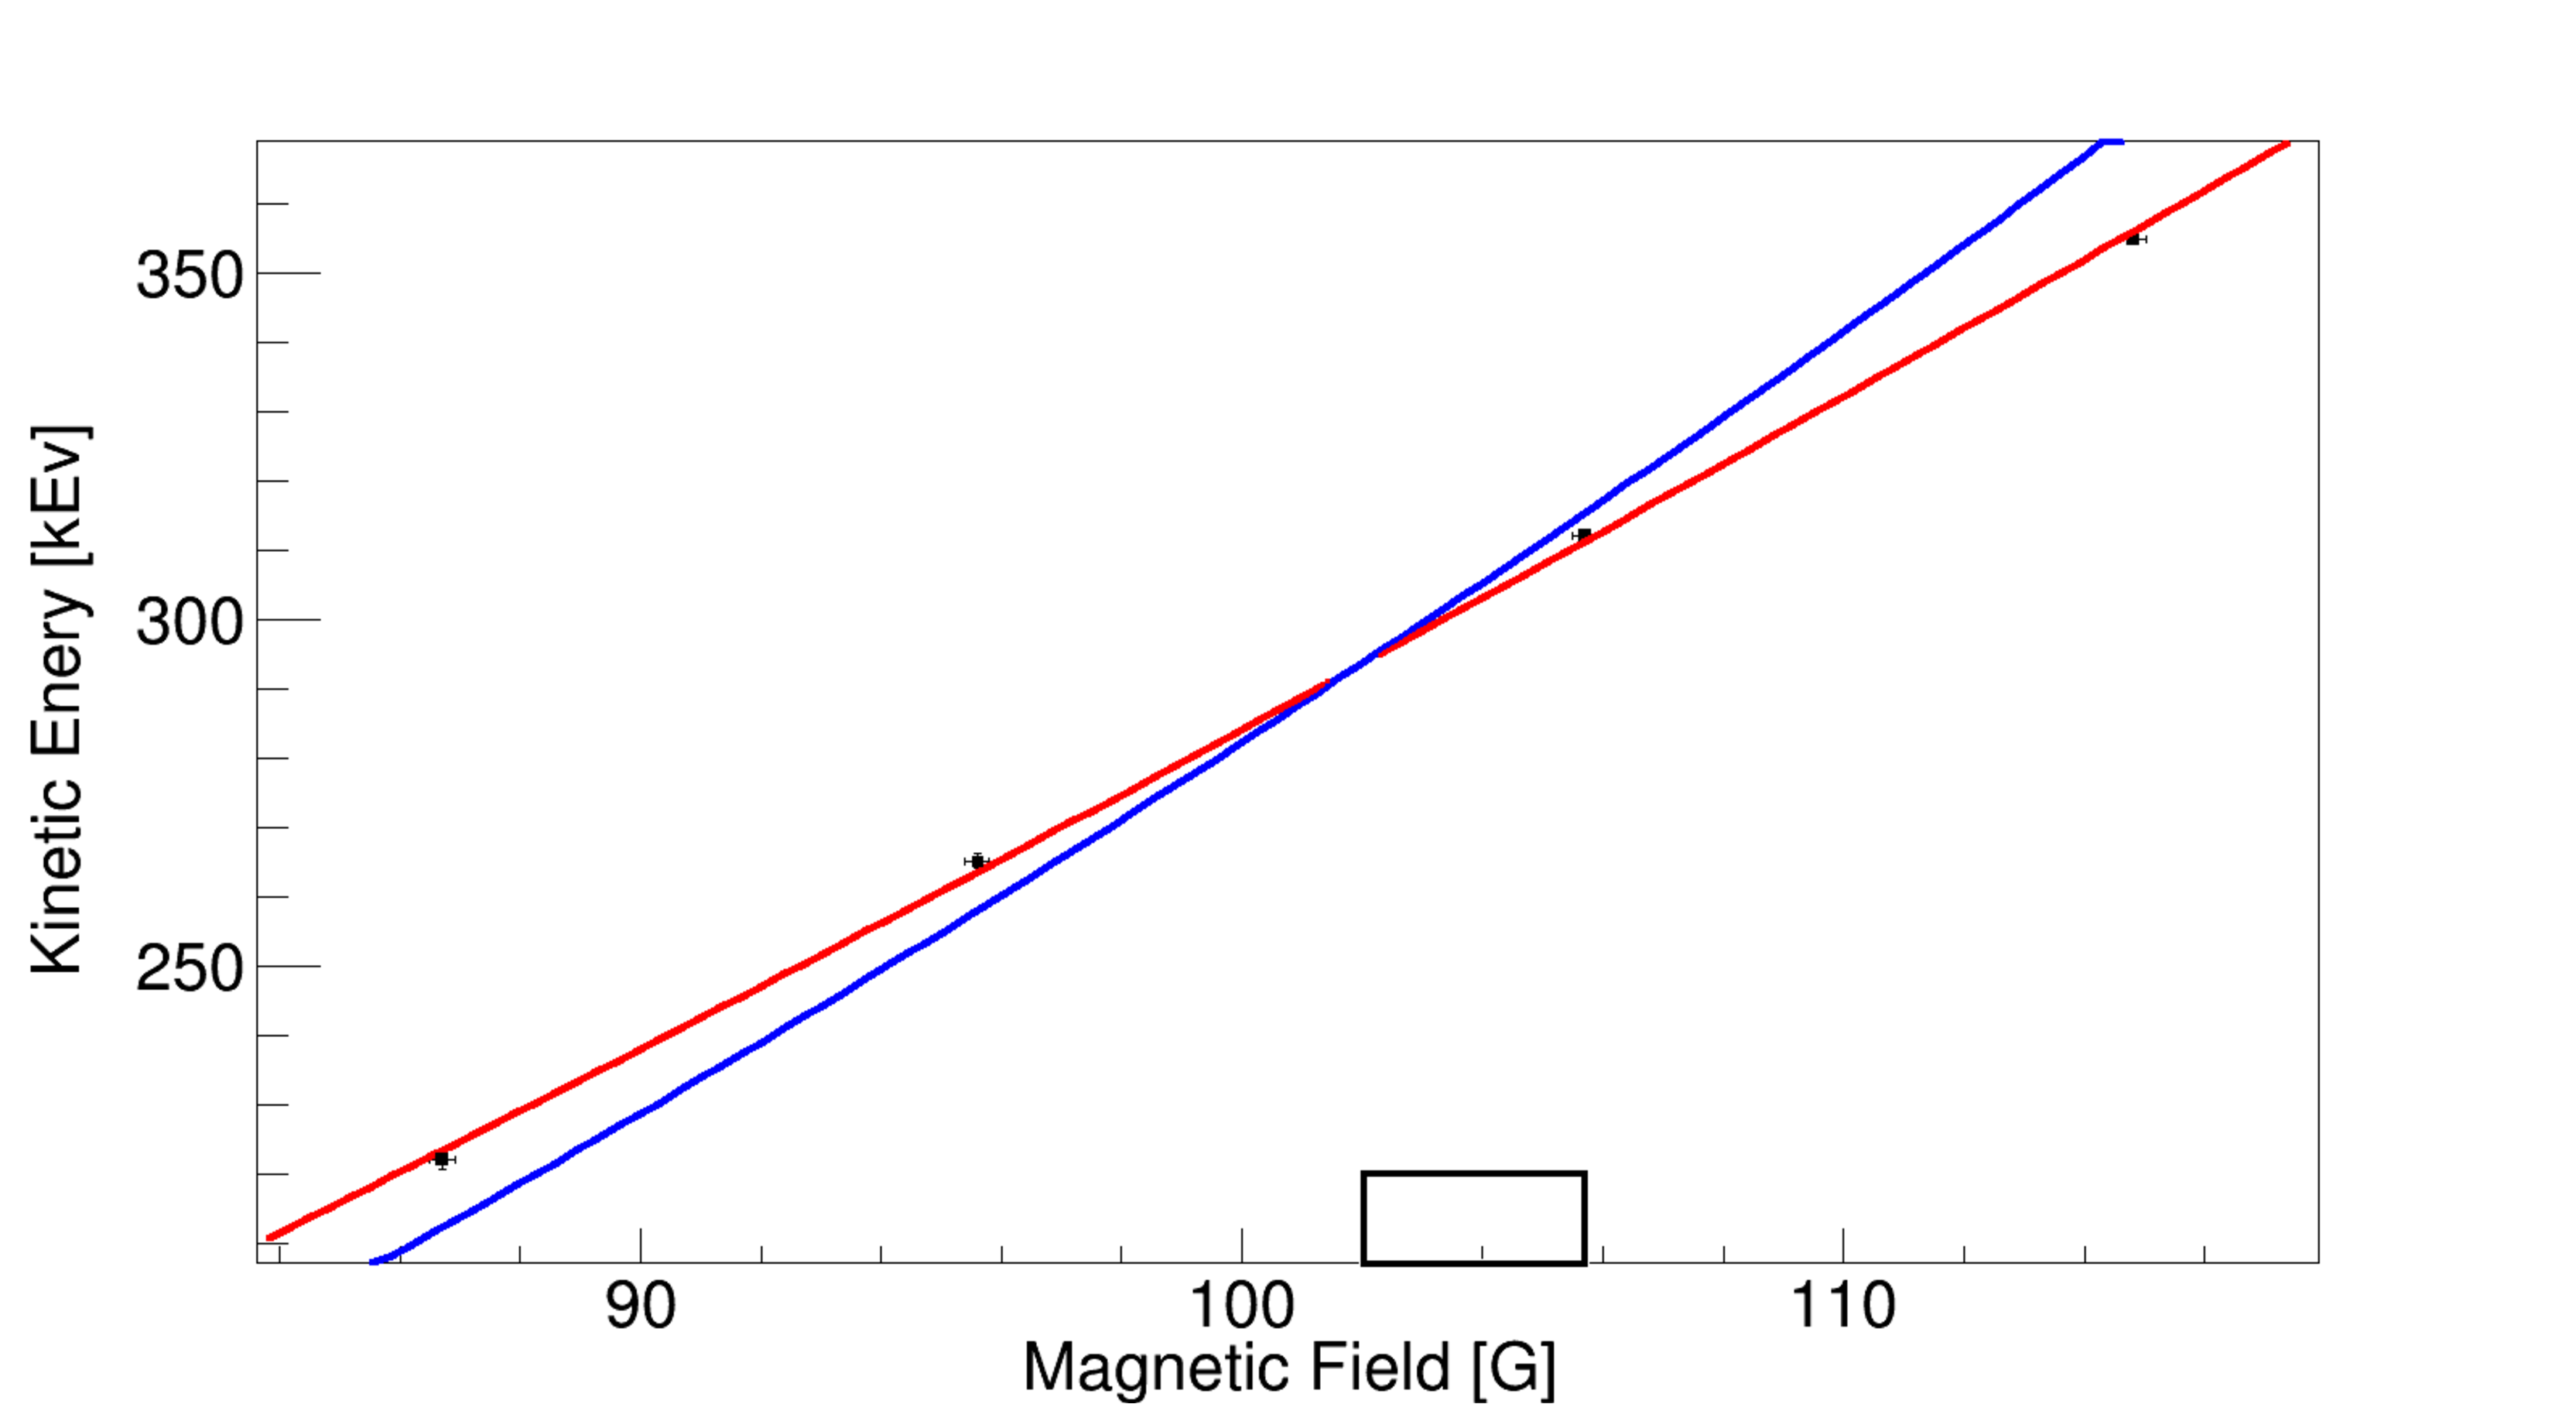
\includegraphics[width=.5\textwidth]{sysgraphpaper.pdf}
  \caption{The four data points acquired in our analysis. At each individual point, the uncorrelated uncertainties from our kinetic energy calculations and our magnetic field averaging is shown. A bar is displayed on the bottom, representing the correlated uncertainty in our magnetic field - i.e, how far all the points could shift horizontally. The relativistic and classical fits are shown in red and blue, respectively.}
  \label{sys}
\end{figure}

Our final four data points, along with the fits described by the two equations $(5)$ and $(6)$, are displayed in Figure \ref{sys}. In order to account for our correlated uncertainties, we fit using a modified version of a chi-squared fit, known as a ``pull" method, detailed in \cite{sys}. This pull method gives us a fit value similar to a reduced chi-squared. For the relativistic fit, this value is $.05$, and for the classical fit, $33.02$. While a reduced chi-squared (or this chi-squared equivalent) less than $1$ can be a sign of overfitting or incorrect error bars, inspecting the fit shows that the relativistic model simply happens to pass through all the points near-perfectly. Our two models cannot be directly compared through standard methods such as Sequential Chi-Square Difference Tests \cite{diff} as neither of the models are nested in the other. However, we can see that the relativistic fit does a better job of capturing the near-linearity of our data.

Using the fit to our relativistic equation, given by Equation $(6)$, we can use the parameters calculated by the fit to determine the electron charge, $e$, and the electron rest energy, $mc^2$. These values, along with the commonly-accepted values in physics literature, are displayed in Table \ref{data}. Both of our values fall within one standard deviation of the expected values.

Our uncertainty of the electron rest mass is a larger proportion of our reported value than our electron charge. A major factor in this is the behavior of the equation we use to fit our data. We expect our relativistic $K(B)$ equation to become approximately linear when the first term, $e^2 \rho^2 B^2$, dominates the second term, $(mc^2)^2$. While this allows for distinguishing between relativistic and classical predictions, the electron rest energy will have a small effect on our data, and as such will not be able to be determined with a great deal of accuracy. This qualitative argument is carried out more rigorously in Appendix B. One would expect our uncertainty in the electron rest mass to be reduced by taking measurements at lower magnetic fields.
\begin{table}[h]
  \begin{ruledtabular}
    \begin{tabular}{ccc}
      &  Measured Values & Expected Values \\
      \hline
      $e$ (esu) & $(5.0 \pm 0.3) \times 10^{-10}$ & $4.8 \times 10^{-10}$ \\
      $mc^2$ (kEv) & $(5.1 \pm 0.76) \times 10^2$ & $5.11 \times 10^2$ \\
      $m$ (g) & $(1.0 \pm 0.23) \times 10^{-27}$ & $0.91 \times 10^{-27}$ \\
    \end{tabular}
  \end{ruledtabular}
  \caption{A comparison of the physical constants predicted by our data and their expected values.}
  \label{data}
\end{table}


In addition to the kinetic energy measured, we can also examine the number of counts detected by the MCA as a function of the electric field supplied to the velocity selector at a given magnetic field. Fitting these distributions to Gaussians and extracting the mean from this distribution, we are able to determine the approximate velocities of our electrons at given magnetic fields. Fitting these data points to relativistic relations gives us the electron charge/mass ratio as $(4.69 \pm 0.96) \times 10^{17}$ esu/g. Putting this relation together with our measurement of the electron charge gives a prediction of the electron mass within one standard deviation of the expected value, displayed in Table \ref{data}.

\section{Conclusion}
By using electromagnetic relations, we are able to accurately determine the momentum, kinetic energy, and velocity of electrons emitted from a $^{90}$Sr/$^{90}$Y source. By comparing our data to the classical and relativistic predictions, we are able to conclude that the theory of special relativity more accurately predicts electron behavior at high speeds. In addition, we are able to determine the electron charge, rest mass, and mass within one standard deviation of expected values. % as $(5.0 \pm 0.3) \times 10^{-10}$ esu, the electron rest energy as $(5.1 \pm 0.76) \times 10^2$ kEv, and the electron mass as $(1.0 \pm 0.23) \times 10^{-27}$ g.

\section{Acknowledgements}
I would like to thank my lab partner, Adin Hrnjic, for providing valuable assistance throughout the experiment. Additionally, I would like to thank Professor Joseph Formaggio for his advice regarding uncertainty propagation. 


\bibliography{dynamics-paper}

\clearpage
\appendix
\section{Reduction of Relativistic Kinetic Energy to Classical Predictions}
Consider the relativistic kinetic energy of a particle,
\begin{equation}
  K = \sqrt{p^2 c^2 + (mc^2)^2} - mc^2
\end{equation}
This equation can be rewritten as
\begin{equation}
  K = mc^2 \sqrt{1 + \left(\frac{p}{mc}\right)^2} - mc^2
\end{equation}
If $pc \ll mc^2$, then $p \ll mc$ and our equation can be expanded to first order as
\begin{equation}
  K \approx  mc^2 \left(1 + \frac{1}{2} \left(\frac{p}{mc}\right)^2 \right) - mc^2 = \frac{p^2}{2m}
\end{equation}
which is our classical equation of kinetic energy.

\section{Error Dependency of $mc^2$ and $e$}
Given 
\begin{equation}
  K = \sqrt{e^2 \rho^2 B^2 - (mc^2)^2} - mc^2
\end{equation}
we wish to determine how errors in $B$ and $K$ will affect the uncertainties in the obtained values of $mc^2$ and $e$. Solving Equation 6 for the two values, we obtain
\begin{equation}
    mc^2 = \frac{B^2 e^2 \rho^2}{2K} - \frac{K}{2}
  \end{equation}
  And
  \begin{equation}
    e = \sqrt{\frac{K^2 + 2Kmc^2}{B^2 \rho^2}}
  \end{equation}
  Standard error propagation is given for some function $f(x,y)$ in first order as
  \begin{equation}
    \sigma_f^2 = \sigma_x^2 \left(\pdv{f}{x}\right)^2 + \sigma_y^2 \left(\pdv{f}{y}\right)^2
  \end{equation}
  This equation assumes that the uncertainties in $B$ and $K$ are uncorrelated, which we expect in our case - fluctuations in the magnetic field and variances in the kinetic energy measured are due to different aspects of our apparatus. As such, the equations for the uncertainty in $mc^2$ and $e$ to first order are given as
  \begin{equation}
    \sigma_{mc^2}^2 = \sigma_B^2 \left(\frac{B \rho^2 e^2}{K}\right)^2 + \left(\frac{\beta^2 e^2 \rho^2}{2K^2} + \frac{1}{c}\right)^2 \sigma_K^2 
  \end{equation}
  and
  \begin{equation}
    \begin{aligned}
    \sigma_e^2 &= \sigma_B^2 \left(\frac{2(K^2 + 2Kmc^2)}{B^4 \rho^6}\right) 
    \\
    &+ \sigma_K^2 \left(\frac{(2K + 2 mc^2)^2}{(K^2 + 2Kmc^2)B^2 \rho^2}\right)
  \end{aligned}
\end{equation}
These equations show that uncertainty in $mc^2$ scales roughly linearly in $B/K$, which we expect to be large in our realm of measurement. This is not so for the uncertainty in $e$, which we expect to scale with terms such as $K/B$ and $K/B^2$. Although this analysis assumes a direct algebraic propagation of errors, as opposed to the propagation of errors to fit parameters through chi-squared and other fitting methods, the mechanism of propagation is similar enough that we can expect a similar scaling argument to hold.




%%%%%%%%%%%%%%%%%%%%%%%%%%%%%%%%%%%%%%%%%%%%%%%%%%%%%%%%%%%%%%%%%%


\end{document}
